\documentclass[11pt]{article}
\usepackage[margin=1in]{geometry}
\usepackage{amsmath, amssymb, amsthm}
\usepackage{algorithm, algpseudocode}
\usepackage{graphicx}
\usepackage{xcolor}
\usepackage{listings}
\usepackage{hyperref}
\usepackage{booktabs}
\usepackage{float}

\definecolor{codegreen}{rgb}{0.2,0.6,0.2}
\definecolor{codered}{rgb}{0.7,0.15,0.15}
\definecolor{codegray}{rgb}{0.4,0.4,0.4}
\definecolor{codebg}{rgb}{0.97,0.97,0.97}

\lstset{
  language=R,
  basicstyle=\ttfamily\small,
  keywordstyle=\color{codered}\bfseries,
  commentstyle=\color{codegray}\itshape,
  stringstyle=\color{codegreen},
  backgroundcolor=\color{codebg},
  frame=single,
  rulecolor=\color{codegray!40},
  numbers=left,
  numberstyle=\tiny\color{codegray},
  breaklines=true,
  columns=fullflexible,
  showstringspaces=false,
  tabsize=2,
  xleftmargin=1.5em,
  framexleftmargin=1em,
}

\newcommand{\R}{\textsf{R}}

\title{Gibbs Sampling: Theory and Implementation}
\author{Adam Kurth \\ PHP 2530 --- Bayesian Statistics}
\date{Spring 2026}

\begin{document}
\maketitle

% ----------------------------------------------------------------
\section{Motivation}

In rejection sampling, we draw exact independent samples from a target~$f$ by bounding it with an envelope~$c\cdot g$.  In importance sampling, we draw from a proposal~$q$ and reweight.  Both methods break down in high dimensions: rejection sampling suffers from exponentially small acceptance rates, and importance sampling suffers from weight collapse (a few particles dominate the entire estimate).

The root problem is that both methods treat the target as a \emph{monolithic} density and try to approximate it with a single proposal.  \textbf{Gibbs sampling} takes a fundamentally different approach: instead of sampling from the full joint distribution~$p(\boldsymbol{\theta} \mid y)$ all at once, it breaks the problem into a sequence of \textbf{univariate conditional draws}.  If the parameter vector is $\boldsymbol{\theta} = (\theta_1, \ldots, \theta_d)$, Gibbs sampling cycles through each component~$\theta_j$ and draws from its \textbf{full conditional distribution}
\[
  p(\theta_j \mid \theta_1, \ldots, \theta_{j-1}, \theta_{j+1}, \ldots, \theta_d, \, y),
\]
holding all other parameters fixed at their current values.  Each of these draws is a one-dimensional problem---often available in closed form for conjugate models---yet the resulting sequence of $d$-dimensional vectors forms a Markov chain whose stationary distribution is the full joint posterior~$p(\boldsymbol{\theta} \mid y)$.

This idea, introduced by Geman and Geman (1984) for image processing and popularized in statistics by Gelfand and Smith (1990), is one of the most widely used MCMC algorithms in Bayesian computation.  BDA3 (Gelman et al., Chapter~11) presents Gibbs sampling as the foundation for practical posterior simulation, especially in hierarchical models where the conditional structure is naturally available.

% ----------------------------------------------------------------
\section{The Algorithm}

\subsection{Systematic-Scan Gibbs Sampler}

\begin{algorithm}[H]
\caption{Gibbs Sampling}
\label{alg:gibbs}
\begin{algorithmic}[1]
\State Initialize $\boldsymbol{\theta}^{(0)} = (\theta_1^{(0)}, \theta_2^{(0)}, \ldots, \theta_d^{(0)})$
\For{$t = 1, 2, \ldots, T$}
  \State Draw $\theta_1^{(t)} \sim p(\theta_1 \mid \theta_2^{(t-1)}, \theta_3^{(t-1)}, \ldots, \theta_d^{(t-1)}, \, y)$
  \State Draw $\theta_2^{(t)} \sim p(\theta_2 \mid \theta_1^{(t)}, \theta_3^{(t-1)}, \ldots, \theta_d^{(t-1)}, \, y)$
  \State \hspace{1em} $\vdots$
  \State Draw $\theta_d^{(t)} \sim p(\theta_d \mid \theta_1^{(t)}, \theta_2^{(t)}, \ldots, \theta_{d-1}^{(t)}, \, y)$
\EndFor
\end{algorithmic}
\end{algorithm}

Note the \emph{within-iteration updating}: when drawing $\theta_j^{(t)}$, we condition on the \textbf{most recent} values of all other components---using $\theta_k^{(t)}$ for $k < j$ (already updated this iteration) and $\theta_k^{(t-1)}$ for $k > j$ (not yet updated).  This is the \textbf{systematic scan} variant.

An alternative is the \textbf{random scan}, where at each iteration a component~$j$ is chosen uniformly at random from $\{1, \ldots, d\}$ and only that component is updated.  Both variants produce valid Markov chains with the correct stationary distribution, but the systematic scan is more common in practice.

\subsection{Why It Works}

The key insight is that each conditional draw leaves the joint distribution invariant.  We formalize this as follows.

\begin{proof}[\textbf{Invariance of the joint distribution}]
Suppose $\boldsymbol{\theta}^{(t)} \sim p(\boldsymbol{\theta} \mid y)$.  Consider the update of component~$j$:
\[
  \theta_j^{(t+1)} \sim p(\theta_j \mid \boldsymbol{\theta}_{-j}^{(t)}, y).
\]
The joint density of $(\theta_j^{(t+1)}, \boldsymbol{\theta}_{-j}^{(t)})$ is
\[
  p(\theta_j^{(t+1)} \mid \boldsymbol{\theta}_{-j}^{(t)}, y) \cdot p(\boldsymbol{\theta}_{-j}^{(t)} \mid y)
  = \frac{p(\theta_j^{(t+1)}, \boldsymbol{\theta}_{-j}^{(t)} \mid y)}{p(\boldsymbol{\theta}_{-j}^{(t)} \mid y)} \cdot p(\boldsymbol{\theta}_{-j}^{(t)} \mid y)
  = p(\theta_j^{(t+1)}, \boldsymbol{\theta}_{-j}^{(t)} \mid y).
\]
Thus the updated vector still has joint distribution $p(\boldsymbol{\theta} \mid y)$.  Since each of the $d$ conditional updates preserves the joint, the full Gibbs iteration (all $d$ updates in sequence) also preserves~$p(\boldsymbol{\theta} \mid y)$.  By the ergodic theorem for Markov chains, the chain converges to this stationary distribution regardless of the starting point, provided mild regularity conditions hold (the chain must be irreducible and aperiodic, which is guaranteed when the full conditionals have everywhere-positive density).
\end{proof}

\subsection{Connection to Metropolis--Hastings}

Gibbs sampling is a special case of the Metropolis--Hastings (MH) algorithm where the proposal is the full conditional distribution and the acceptance probability is always~1.

To see this, consider an MH step for component~$j$ with proposal $q(\theta_j^* \mid \boldsymbol{\theta}_{-j}) = p(\theta_j^* \mid \boldsymbol{\theta}_{-j}, y)$.  The acceptance ratio is:
\begin{align*}
  \alpha &= \min\!\left(1, \;\frac{p(\theta_j^*, \boldsymbol{\theta}_{-j} \mid y)}{p(\theta_j, \boldsymbol{\theta}_{-j} \mid y)} \cdot \frac{q(\theta_j \mid \boldsymbol{\theta}_{-j})}{q(\theta_j^* \mid \boldsymbol{\theta}_{-j})}\right) \\[6pt]
  &= \min\!\left(1, \;\frac{p(\theta_j^*\mid\boldsymbol{\theta}_{-j},y)\,p(\boldsymbol{\theta}_{-j}\mid y)}{p(\theta_j\mid\boldsymbol{\theta}_{-j},y)\,p(\boldsymbol{\theta}_{-j}\mid y)} \cdot \frac{p(\theta_j\mid\boldsymbol{\theta}_{-j},y)}{p(\theta_j^*\mid\boldsymbol{\theta}_{-j},y)}\right) \\[6pt]
  &= \min(1, \; 1) = 1.
\end{align*}
Every proposed move is accepted.  This makes Gibbs sampling maximally efficient \emph{for each component-wise update}---it never wastes a draw.

% ----------------------------------------------------------------
\section{Example 1: Bivariate Normal}

The canonical example for building intuition about Gibbs sampling uses a bivariate normal target.

\subsection{Setup}

Let the target be
\[
  \begin{pmatrix} \theta_1 \\ \theta_2 \end{pmatrix}
  \sim N\!\left(
    \begin{pmatrix} 0 \\ 0 \end{pmatrix},
    \begin{pmatrix} 1 & \rho \\ \rho & 1 \end{pmatrix}
  \right).
\]

\subsection{Full Conditionals}

From the properties of the multivariate normal, the full conditionals are:
\begin{align}
  \theta_1 \mid \theta_2 &\sim N\!\left(\mu_1 + \rho\,\frac{\sigma_1}{\sigma_2}(\theta_2 - \mu_2), \;\; \sigma_1^2(1 - \rho^2)\right) = N(\rho\,\theta_2, \;\; 1 - \rho^2), \label{eq:cond1} \\[4pt]
  \theta_2 \mid \theta_1 &\sim N\!\left(\mu_2 + \rho\,\frac{\sigma_2}{\sigma_1}(\theta_1 - \mu_1), \;\; \sigma_2^2(1 - \rho^2)\right) = N(\rho\,\theta_1, \;\; 1 - \rho^2). \label{eq:cond2}
\end{align}

In general, for a bivariate normal $(\theta_1, \theta_2)^\top \sim N(\boldsymbol{\mu}, \Sigma)$ with $\Sigma = \bigl(\begin{smallmatrix} \sigma_1^2 & \rho\sigma_1\sigma_2 \\ \rho\sigma_1\sigma_2 & \sigma_2^2 \end{smallmatrix}\bigr)$, the conditional $\theta_1 \mid \theta_2$ has:
\begin{itemize}
  \item \textbf{Mean}: the best linear predictor $\mu_1 + \rho(\sigma_1/\sigma_2)(\theta_2 - \mu_2)$---the ``regression'' of $\theta_1$ on $\theta_2$.
  \item \textbf{Variance}: $\sigma_1^2(1-\rho^2)$---reduced by a factor $(1-\rho^2)$ compared to the marginal variance.  When $\rho \to 1$, the conditional variance shrinks to zero and each $\theta_1$-update barely moves, causing slow mixing.
\end{itemize}

\subsection{Implementation}

\begin{lstlisting}
gibbs_bivariate <- function(n_iter, rho, init = c(-2, -2)) {
  theta <- matrix(NA, n_iter, 2)
  theta[1, ] <- init
  cond_sd <- sqrt(1 - rho^2)
  for (t in 2:n_iter) {
    # draw theta1 | theta2
    theta[t, 1] <- rnorm(1, rho * theta[t-1, 2], cond_sd)
    # draw theta2 | theta1
    theta[t, 2] <- rnorm(1, rho * theta[t, 1], cond_sd)
  }
  theta
}
\end{lstlisting}

Notice that when drawing $\theta_2^{(t)}$, we use the \emph{just-updated} $\theta_1^{(t)}$, not the old $\theta_1^{(t-1)}$.

\paragraph{Figure~\ref{fig:bivariate}: Gibbs mechanics.}
Panel~(a) shows the ``staircase'' path traced by the Gibbs sampler on the joint density contours: each step moves horizontally ($\theta_1$ update, green) then vertically ($\theta_2$ update, blue).  The zig-zag pattern is characteristic of Gibbs sampling.  Panels~(b) and~(c) show the trace plots for each component converging quickly to the stationary distribution.  Panel~(d) confirms that the marginal histograms match the true $N(0,1)$ density.

\begin{figure}[H]
  \centering
  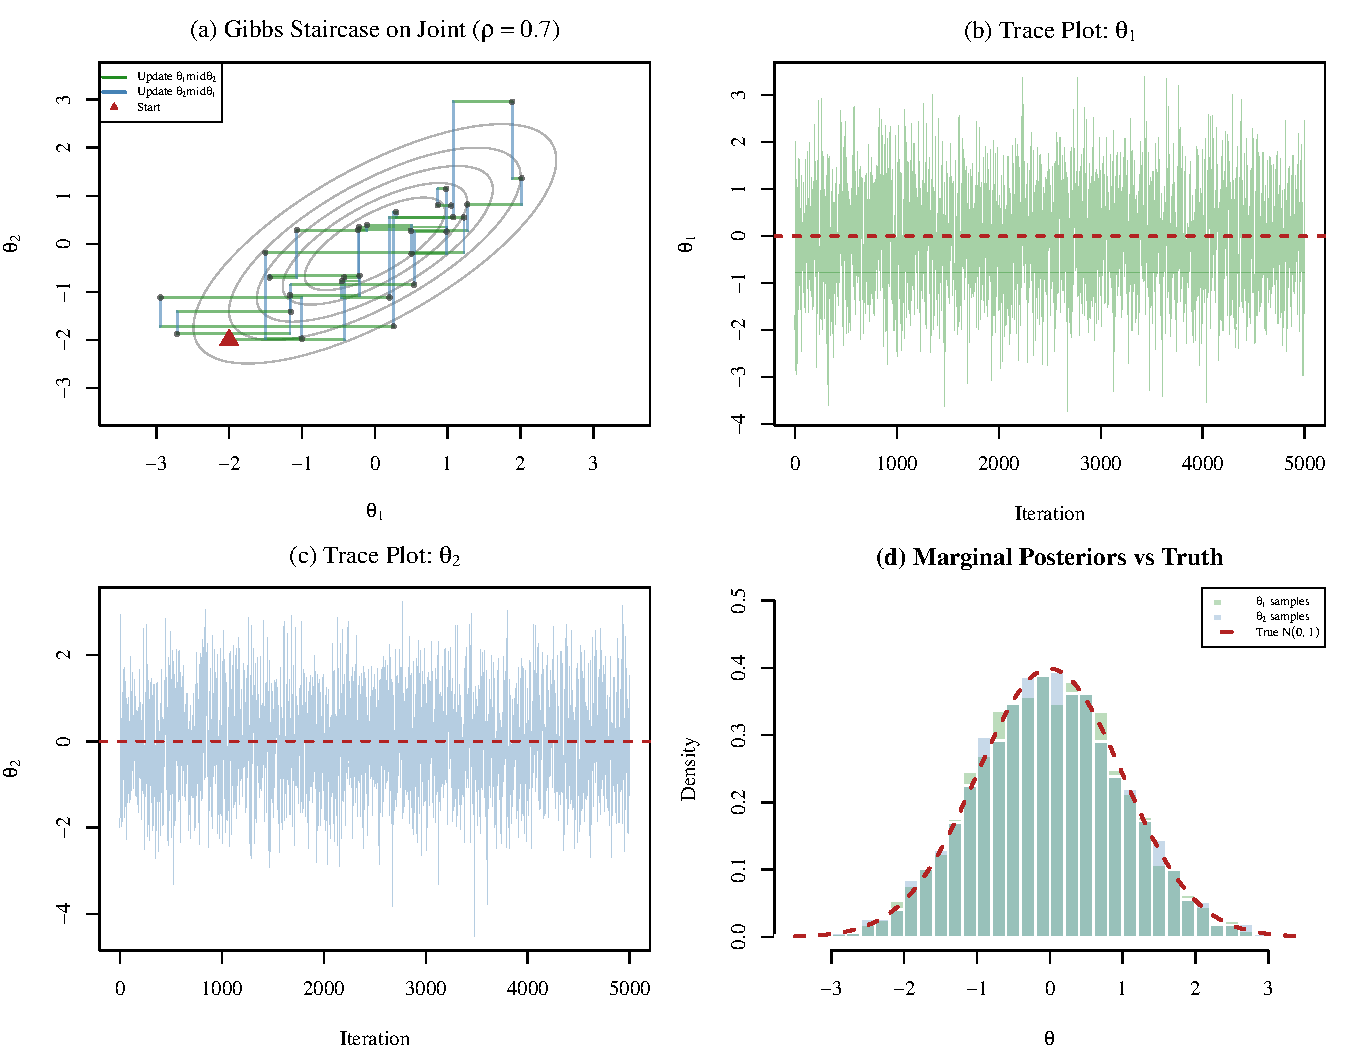
\includegraphics[width=\textwidth]{plots/fig_gibbs_bivariate.pdf}
  \caption{%
    \textbf{(a)}~Gibbs staircase on the joint density contours of a bivariate normal with $\rho = 0.7$.  Green segments update $\theta_1 \mid \theta_2$; blue segments update $\theta_2 \mid \theta_1$.
    \textbf{(b)}~Trace plot of $\theta_1$.
    \textbf{(c)}~Trace plot of $\theta_2$.
    \textbf{(d)}~Marginal histograms vs.\ true $N(0,1)$ density.
  }
  \label{fig:bivariate}
\end{figure}

\paragraph{Figure~\ref{fig:steps}: Step-by-step visualization.}
Six sequential Gibbs iterations are isolated in separate panels.  At each step, the horizontal green segment represents sampling $\theta_1$ from its full conditional (a horizontal ``slice'' through the contour at the current $\theta_2$), and the vertical blue segment represents sampling $\theta_2$ from its conditional.  The orange star marks each new sample.  Previous samples accumulate across panels, showing how the chain builds up its exploration of the target.

\begin{figure}[H]
  \centering
  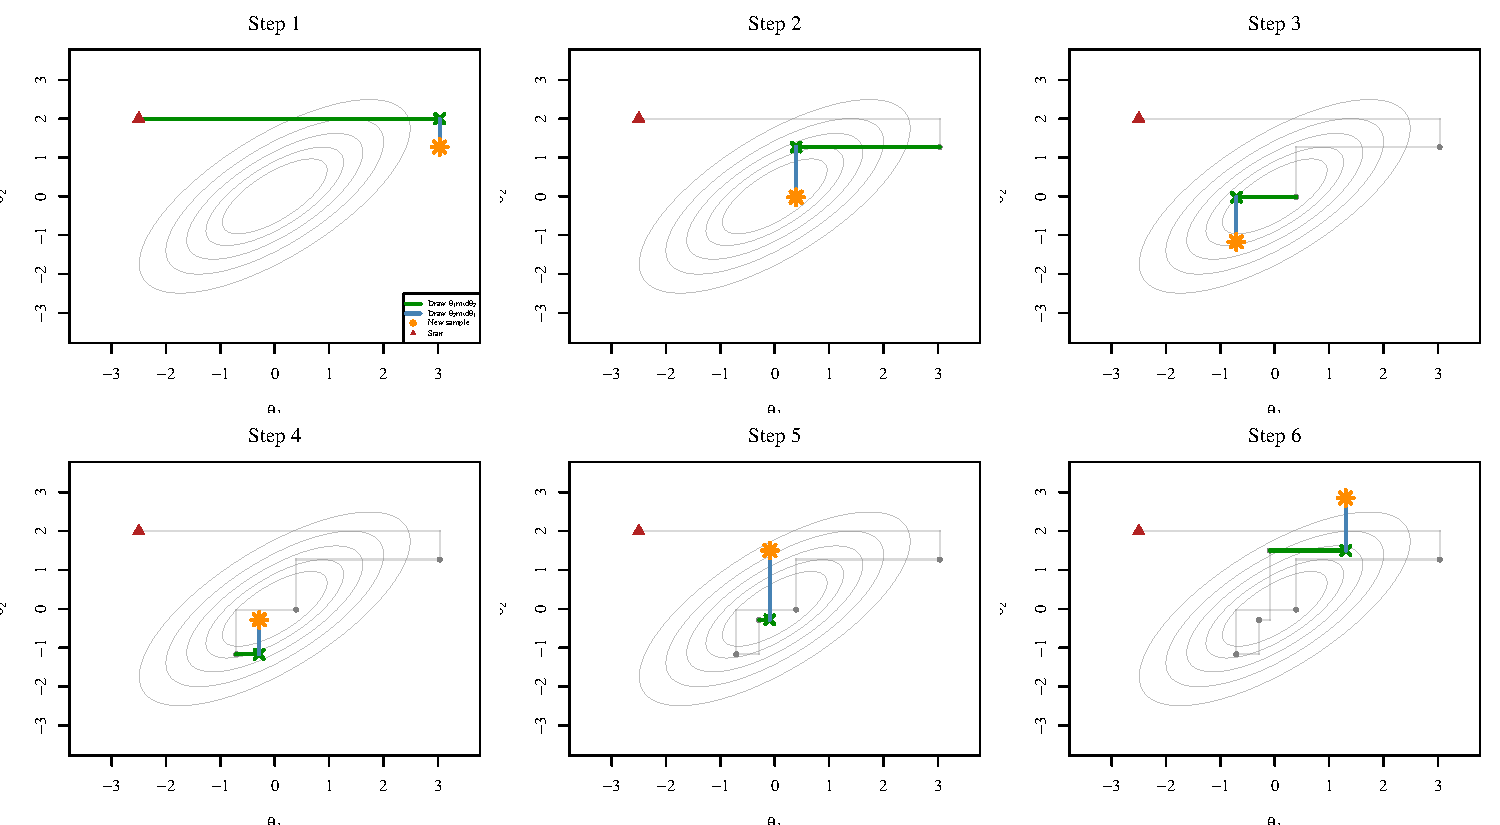
\includegraphics[width=\textwidth]{plots/fig_gibbs_steps.pdf}
  \caption{Six sequential Gibbs iterations for the bivariate normal.  Each panel adds one iteration: green = $\theta_1 \mid \theta_2$ update, blue = $\theta_2 \mid \theta_1$ update, orange star = new sample, red triangle = starting point.  The characteristic horizontal--vertical staircase emerges.}
  \label{fig:steps}
\end{figure}

% ----------------------------------------------------------------
\section{The Role of Correlation: Why Gibbs Slows Down}

The bivariate normal example reveals a fundamental limitation of Gibbs sampling.  Because Gibbs updates are \textbf{axis-aligned}---each step moves along one coordinate axis---the sampler can only explore diagonally-oriented structure through a sequence of small horizontal and vertical increments.

\subsection{Quantifying the Slowdown}

For the bivariate normal with correlation~$\rho$, the \textbf{lag-1 autocorrelation} of the Gibbs chain is exactly $\rho^2$ (Amit, 1991; Liu, 2001).  This means:
\begin{itemize}
  \item At $\rho = 0.2$: autocorrelation $= 0.04$, the chain mixes almost as fast as i.i.d.\ sampling.
  \item At $\rho = 0.7$: autocorrelation $= 0.49$, consecutive samples are moderately correlated.
  \item At $\rho = 0.95$: autocorrelation $= 0.9025$, consecutive samples are nearly identical---the chain ``crawls'' along the major axis of the ellipse.
\end{itemize}

The \textbf{effective sample size} (ESS) is approximately
\[
  n_{\text{eff}} \approx \frac{T}{1 + 2\sum_{k=1}^{\infty} \rho^{2k}} = \frac{T(1 - \rho^2)}{1 + \rho^2},
\]
where $T$ is the total number of iterations.  At $\rho = 0.95$, ESS is about $2.6\%$ of~$T$.

\paragraph{Figure~\ref{fig:correlation}: Correlation effect on mixing.}
Panels~(a)--(c) show the Gibbs staircase for $\rho = 0.2$, $0.7$, and $0.95$.  As $\rho$ increases, the staircase becomes increasingly confined to a narrow diagonal band and the sampler takes many iterations to traverse the distribution.  Panel~(d) shows the autocorrelation function: for $\rho = 0.95$, significant autocorrelation persists beyond lag~50.

\begin{figure}[H]
  \centering
  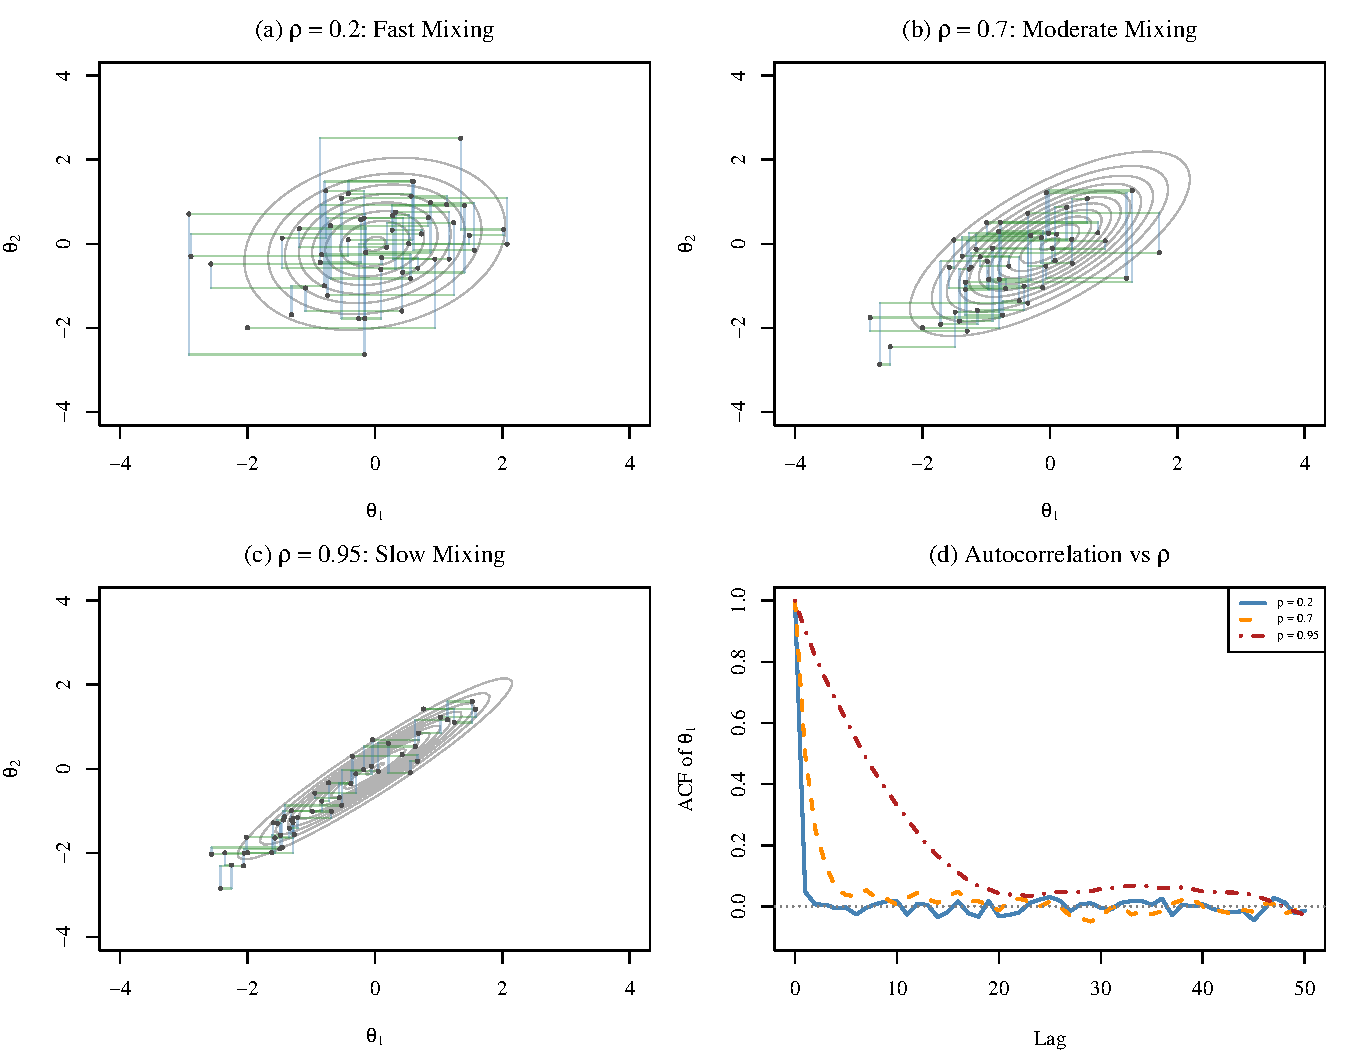
\includegraphics[width=\textwidth]{plots/fig_gibbs_correlation.pdf}
  \caption{%
    \textbf{(a)}~$\rho = 0.2$: fast mixing, broad staircase.
    \textbf{(b)}~$\rho = 0.7$: moderate mixing.
    \textbf{(c)}~$\rho = 0.95$: slow mixing, tight zig-zag.
    \textbf{(d)}~Autocorrelation decays slowly with increasing $\rho$.
  }
  \label{fig:correlation}
\end{figure}

% ----------------------------------------------------------------
\section{Example 2: Bayesian Normal Model}

We now apply Gibbs sampling to a genuine Bayesian inference problem: estimating both the mean and variance of a normal distribution from data.

\subsection{Model}

\begin{align*}
  y_i \mid \mu, \sigma^2 &\sim N(\mu, \sigma^2), \quad i = 1, \ldots, n, \\
  \mu &\sim N(\mu_0, \tau_0^2), \\
  \sigma^2 &\sim \text{Inv-}\chi^2(\nu_0, \sigma_0^2).
\end{align*}

Here the Inverse-$\chi^2$ prior on $\sigma^2$ is parameterized so that $E[\sigma^2] = \nu_0 \sigma_0^2 / (\nu_0 - 2)$ for $\nu_0 > 2$.  This is the standard conjugate setup from BDA3, Chapter~3.

\subsection{Full Conditionals}

\paragraph{$\mu \mid \sigma^2, y$.}
The likelihood contributes $\sum_i (y_i - \mu)^2 / (2\sigma^2)$ to the log-posterior, and the prior contributes $(\mu - \mu_0)^2 / (2\tau_0^2)$.  Completing the square gives:
\[
  \mu \mid \sigma^2, y \sim N\!\left(\frac{n\bar{y}/\sigma^2 + \mu_0/\tau_0^2}{n/\sigma^2 + 1/\tau_0^2}, \;\; \frac{1}{n/\sigma^2 + 1/\tau_0^2}\right).
\]
The posterior mean is a \textbf{precision-weighted average} of the prior mean~$\mu_0$ and the sample mean~$\bar{y}$, with precisions $1/\tau_0^2$ and $n/\sigma^2$ respectively.  When the prior is vague ($\tau_0^2 \to \infty$), the posterior mean converges to~$\bar{y}$ and the posterior variance to $\sigma^2/n$.

\paragraph{$\sigma^2 \mid \mu, y$.}
With the Inverse-$\chi^2$ prior:
\[
  \sigma^2 \mid \mu, y \sim \text{Inv-}\chi^2\!\left(\nu_0 + n, \;\; \frac{\nu_0 \sigma_0^2 + \sum_{i=1}^n (y_i - \mu)^2}{\nu_0 + n}\right).
\]
Equivalently, sampling $\sigma^2 \sim \text{Inv-}\chi^2(\nu_n, s_n^2)$ is done by drawing $X \sim \text{Gamma}(\nu_n/2, \; \nu_n s_n^2/2)$ and setting $\sigma^2 = 1/X$.  The posterior degrees of freedom $\nu_n = \nu_0 + n$ combine the prior and sample information, and the posterior scale $s_n^2$ is a weighted combination of the prior scale and the sum of squared deviations from the current~$\mu$.

\begin{lstlisting}
for (t in 2:n_gibbs) {
  # mu | sigma^2, y
  prec <- n / sigma2[t-1] + 1 / tau0_sq
  cond_mean <- (n * ybar / sigma2[t-1] + mu0 / tau0_sq) / prec
  mu[t] <- rnorm(1, cond_mean, sqrt(1 / prec))

  # sigma^2 | mu, y ~ Inv-Chi^2(nu_n, s_n^2)
  nu_n <- nu0 + n
  ss <- sum((y - mu[t])^2)
  s_n <- (nu0 * sigma0_sq + ss) / nu_n
  sigma2[t] <- 1 / rgamma(1, nu_n / 2, rate = nu_n * s_n / 2)
}
\end{lstlisting}

\paragraph{Figure~\ref{fig:normal}: Gibbs applied to the normal model.}
We simulated $n = 30$ observations from $N(5, 4)$ and ran 10,000 Gibbs iterations with vague priors ($\mu_0 = 0$, $\tau_0^2 = 100$, $\nu_0 = 1$, $\sigma_0^2 = 1$).  The chain converges rapidly.  Panel~(c) shows the joint posterior samples with a few staircase iterations overlaid.  Panel~(d) shows the marginal posterior of~$\mu$ centered near $\bar{y} \approx 5.14$, confirming that vague priors let the data dominate.

\begin{figure}[H]
  \centering
  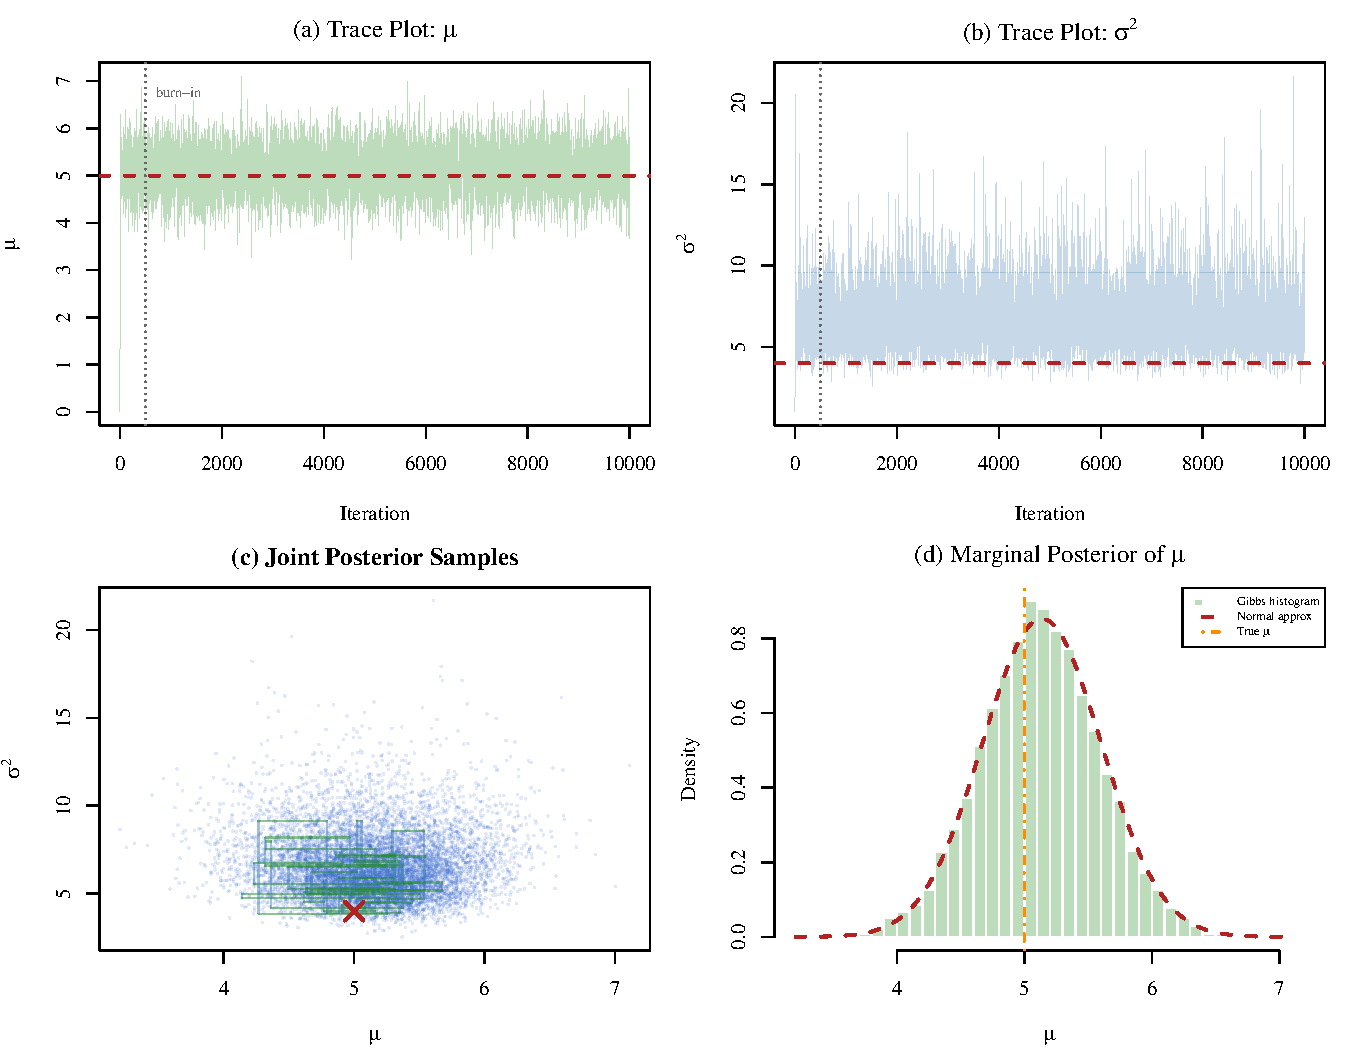
\includegraphics[width=\textwidth]{plots/fig_gibbs_normal_model.pdf}
  \caption{%
    \textbf{(a)}~Trace of $\mu$ (true value = 5, dashed red).
    \textbf{(b)}~Trace of $\sigma^2$ (true value = 4).
    \textbf{(c)}~Joint posterior samples with Gibbs path overlay.
    \textbf{(d)}~Marginal posterior of $\mu$ (histogram) vs.\ normal approximation.
  }
  \label{fig:normal}
\end{figure}

% ----------------------------------------------------------------
\section{Example 3: Hierarchical Normal Model}

Hierarchical models are where Gibbs sampling truly shines.  The multi-level conditional structure maps directly onto the Gibbs updates, and the resulting sampler is often straightforward to implement even when the joint posterior is analytically intractable.

\subsection{The ``Eight Schools'' Model (BDA3, Chapter 5)}

The classic example from Rubin (1981) and BDA3 involves $J = 8$ schools that each ran a coaching program.  The observed treatment effects $y_j$ and their standard errors $\sigma_j$ (treated as known) are:

\begin{table}[H]
\centering
\begin{tabular}{lcccccccc}
\toprule
School & A & B & C & D & E & F & G & H \\
\midrule
$y_j$ & 28 & 8 & $-3$ & 7 & $-1$ & 1 & 18 & 12 \\
$\sigma_j$ & 15 & 10 & 16 & 11 & 9 & 11 & 10 & 18 \\
\bottomrule
\end{tabular}
\end{table}

\subsection{Model Specification}

\begin{align*}
  y_j \mid \theta_j &\sim N(\theta_j, \sigma_j^2), \quad j = 1, \ldots, J, \\
  \theta_j \mid \mu, \tau &\sim N(\mu, \tau^2), \\
  \mu &\sim N(0, 10^4), \quad \tau^2 \sim \text{Inv-}\chi^2(1, 1).
\end{align*}

The key feature is \textbf{partial pooling}: the school-level effects $\theta_j$ are neither treated as completely independent (no pooling, $\hat{\theta}_j = y_j$) nor forced to be equal (complete pooling, $\hat{\theta}_j = \bar{y}$).  Instead, the hierarchical prior $\theta_j \sim N(\mu, \tau^2)$ \emph{shrinks} the individual estimates toward the group mean~$\mu$, with the degree of shrinkage governed by~$\tau$.

\subsection{Full Conditionals}

\paragraph{$\theta_j \mid \mu, \tau^2, y_j$.}
Each $\theta_j$ has its own conjugate update:
\[
  \theta_j \mid \mu, \tau^2, y_j \sim N\!\left(\frac{y_j/\sigma_j^2 + \mu/\tau^2}{1/\sigma_j^2 + 1/\tau^2}, \;\; \frac{1}{1/\sigma_j^2 + 1/\tau^2}\right).
\]
The posterior mean is a precision-weighted average of the data $y_j$ (precision $1/\sigma_j^2$) and the group mean $\mu$ (precision $1/\tau^2$).  When $\tau$ is small, $\mu$ dominates (strong pooling); when $\tau$ is large, the data dominate (weak pooling).

\paragraph{$\mu \mid \boldsymbol{\theta}, \tau^2$.}
Conditional on all $\theta_j$ and $\tau^2$:
\[
  \mu \mid \boldsymbol{\theta}, \tau^2 \sim N\!\left(\frac{\sum_j \theta_j / \tau^2 + \mu_0/\tau_{\mu}^2}{J/\tau^2 + 1/\tau_{\mu}^2}, \;\; \frac{1}{J/\tau^2 + 1/\tau_{\mu}^2}\right).
\]

\paragraph{$\tau^2 \mid \boldsymbol{\theta}, \mu$.}
With the Inverse-$\chi^2$ prior:
\[
  \tau^2 \mid \boldsymbol{\theta}, \mu \sim \text{Inv-}\chi^2\!\left(\nu_0 + J, \;\; \frac{\nu_0 s_0^2 + \sum_j (\theta_j - \mu)^2}{\nu_0 + J}\right).
\]

\begin{lstlisting}
for (t in 2:n_hier) {
  # 1. Update each theta_j | mu, tau^2, y_j
  for (j in 1:J) {
    prec_j <- 1 / sigma2_j[j] + 1 / tau2[t-1]
    mean_j <- (y[j] / sigma2_j[j] + mu[t-1] / tau2[t-1]) / prec_j
    theta[t, j] <- rnorm(1, mean_j, sqrt(1 / prec_j))
  }
  # 2. Update mu | theta, tau^2
  prec_mu <- J / tau2[t-1] + 1 / mu_prior_var
  mean_mu <- (sum(theta[t, ]) / tau2[t-1]) / prec_mu
  mu[t] <- rnorm(1, mean_mu, sqrt(1 / prec_mu))
  # 3. Update tau^2 | theta, mu
  nu_n <- nu0 + J
  ss <- sum((theta[t, ] - mu[t])^2)
  s_n <- (nu0 * s0_sq + ss) / nu_n
  tau2[t] <- 1 / rgamma(1, nu_n / 2, rate = nu_n * s_n / 2)
}
\end{lstlisting}

\paragraph{Figure~\ref{fig:hierarchical}: Hierarchical model results.}
Panel~(a) shows trace plots for four selected $\theta_j$'s---they mix well.  Panel~(b) shows the posterior of the population mean~$\mu$, centered around 8.  Panel~(c) shows the posterior of~$\tau$---note it is right-skewed and includes substantial mass near zero, reflecting uncertainty about whether the schools truly differ.  Panel~(d) is the \textbf{shrinkage plot}: raw estimates $y_j$ (red crosses) are pulled toward the grand mean (orange dashed line) to produce the posterior means $E[\theta_j \mid y]$ (blue dots with 95\% intervals).  Schools with large standard errors (e.g., School~A with $y_1 = 28$, $\sigma_1 = 15$) are shrunk the most.

\begin{figure}[H]
  \centering
  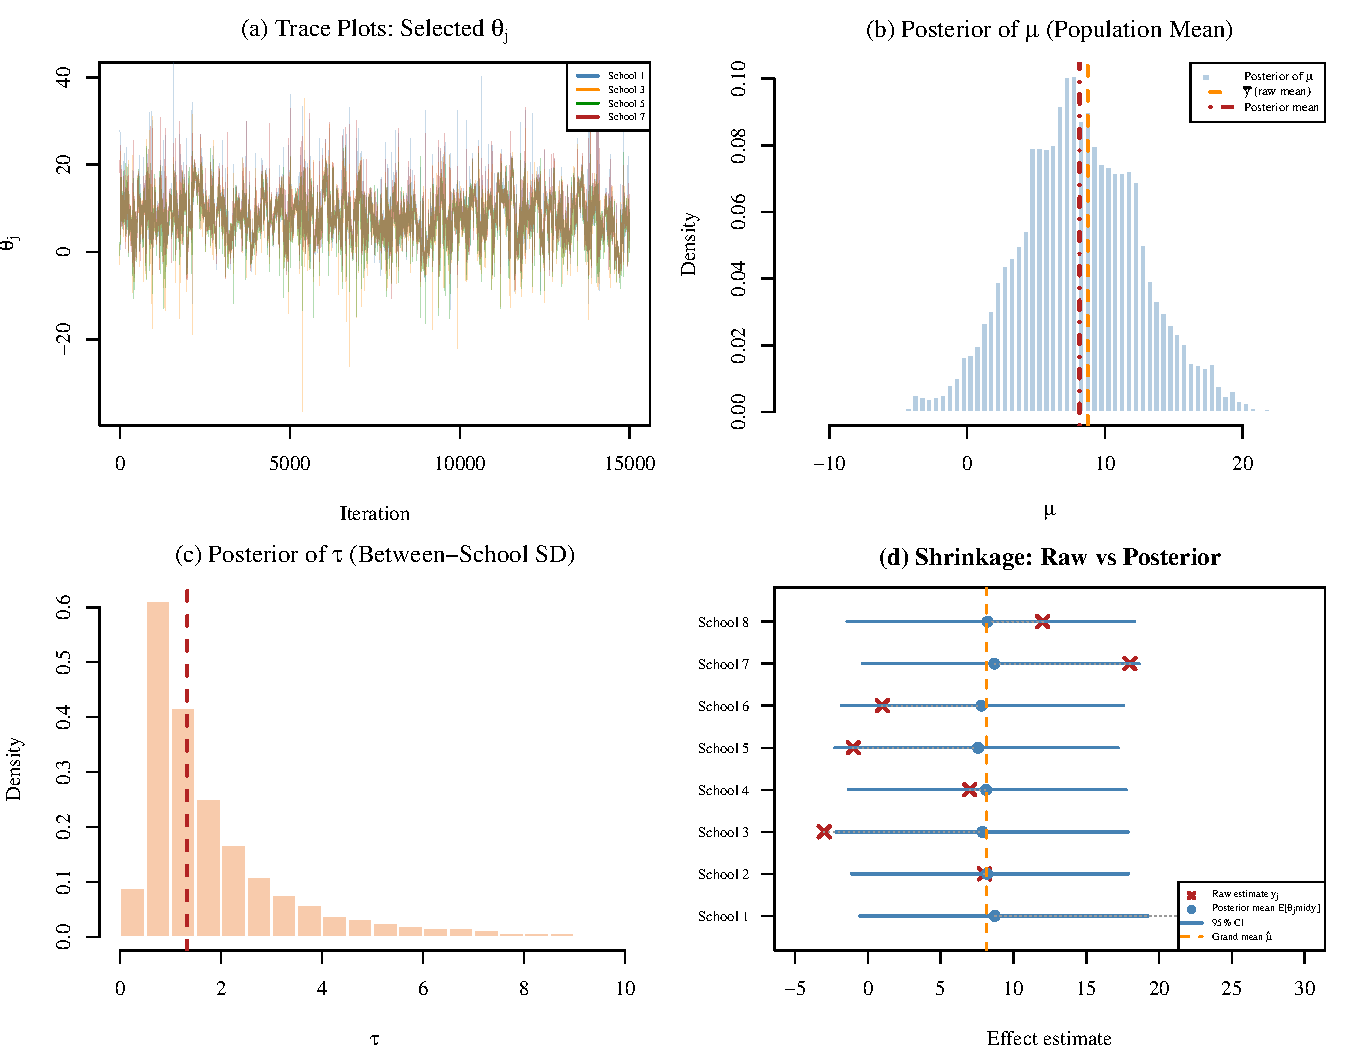
\includegraphics[width=\textwidth]{plots/fig_gibbs_hierarchical.pdf}
  \caption{%
    \textbf{(a)}~Trace plots for $\theta_1, \theta_3, \theta_5, \theta_7$.
    \textbf{(b)}~Posterior of $\mu$ (population mean); raw mean $\bar{y}$ in orange.
    \textbf{(c)}~Posterior of $\tau$ (between-school SD).
    \textbf{(d)}~Shrinkage: raw $y_j$ (red crosses) pulled toward the posterior means (blue dots) with 95\% credible intervals.
  }
  \label{fig:hierarchical}
\end{figure}

% ----------------------------------------------------------------
\section{Convergence Diagnostics}

A Gibbs sampler (or any MCMC method) produces a Markov chain, not i.i.d.\ samples.  We must assess whether the chain has converged to its stationary distribution and how many effectively independent samples it yields.  BDA3, Sections~11.4--11.5, provides a thorough treatment; we summarize the key tools here.

\subsection{Visual Inspection and Burn-In}

The simplest diagnostic is to plot the trace of each parameter.  The initial transient---where the chain migrates from its starting value to the high-density region---must be discarded as \textbf{burn-in}.  A well-mixed chain looks like a ``fuzzy caterpillar'': it oscillates rapidly around a stationary level with no visible trends or drifts.

\subsection{The Gelman--Rubin Diagnostic $\hat{R}$}

BDA3 recommends running $m \ge 2$ chains from \textbf{dispersed starting points} and comparing the within-chain versus between-chain variability.  Let each chain have $n$ post-warmup draws.  Define:
\[
  B = \frac{n}{m-1}\sum_{j=1}^{m}(\bar{\theta}_{j\cdot} - \bar{\theta}_{\cdot\cdot})^2, \qquad
  W = \frac{1}{m}\sum_{j=1}^{m} s_j^2,
\]
where $\bar{\theta}_{j\cdot}$ is the mean of chain~$j$, $\bar{\theta}_{\cdot\cdot}$ the grand mean, and $s_j^2$ the within-chain variance.  The pooled posterior variance estimate is:
\[
  \widehat{\text{var}}^+(\theta \mid y) = \frac{n-1}{n}\,W + \frac{1}{n}\,B,
\]
and the potential scale reduction factor is:
\[
  \hat{R} = \sqrt{\frac{\widehat{\text{var}}^+(\theta \mid y)}{W}}.
\]

If the chains have converged to the same distribution, $B/n \approx 0$ and $\hat{R} \approx 1$.  Large $\hat{R}$ (conventionally $> 1.1$) indicates that the chains have not yet mixed and more iterations are needed.

\subsection{Effective Sample Size}

Even after convergence, consecutive MCMC draws are autocorrelated.  The \textbf{effective sample size} quantifies how many independent samples the chain is worth:
\[
  n_{\text{eff}} = \frac{mn}{1 + 2\sum_{t=1}^{T} \hat{\rho}_t},
\]
where $\hat{\rho}_t$ is the estimated autocorrelation at lag~$t$ and the sum is truncated using an initial monotone sequence estimator (BDA3, p.~287).  For the bivariate normal Gibbs sampler with correlation~$\rho$, $n_{\text{eff}} \approx T(1-\rho^2)/(1+\rho^2)$, confirming the analytic result from Section~4.

\paragraph{Figure~\ref{fig:diagnostics}: Convergence diagnostics.}
We ran 4 chains from dispersed starting points ($(\pm 4, \pm 4)$) on the bivariate normal with $\rho = 0.7$.  Panel~(a) shows the chains converging within $\sim$100 iterations.  Panel~(b) plots the running mean of each chain, which stabilizes near zero.  Panel~(c) shows $\hat{R}$ dropping from its initial inflation to near 1.0.  Panel~(d) shows the autocorrelation function for a single chain.

\begin{figure}[H]
  \centering
  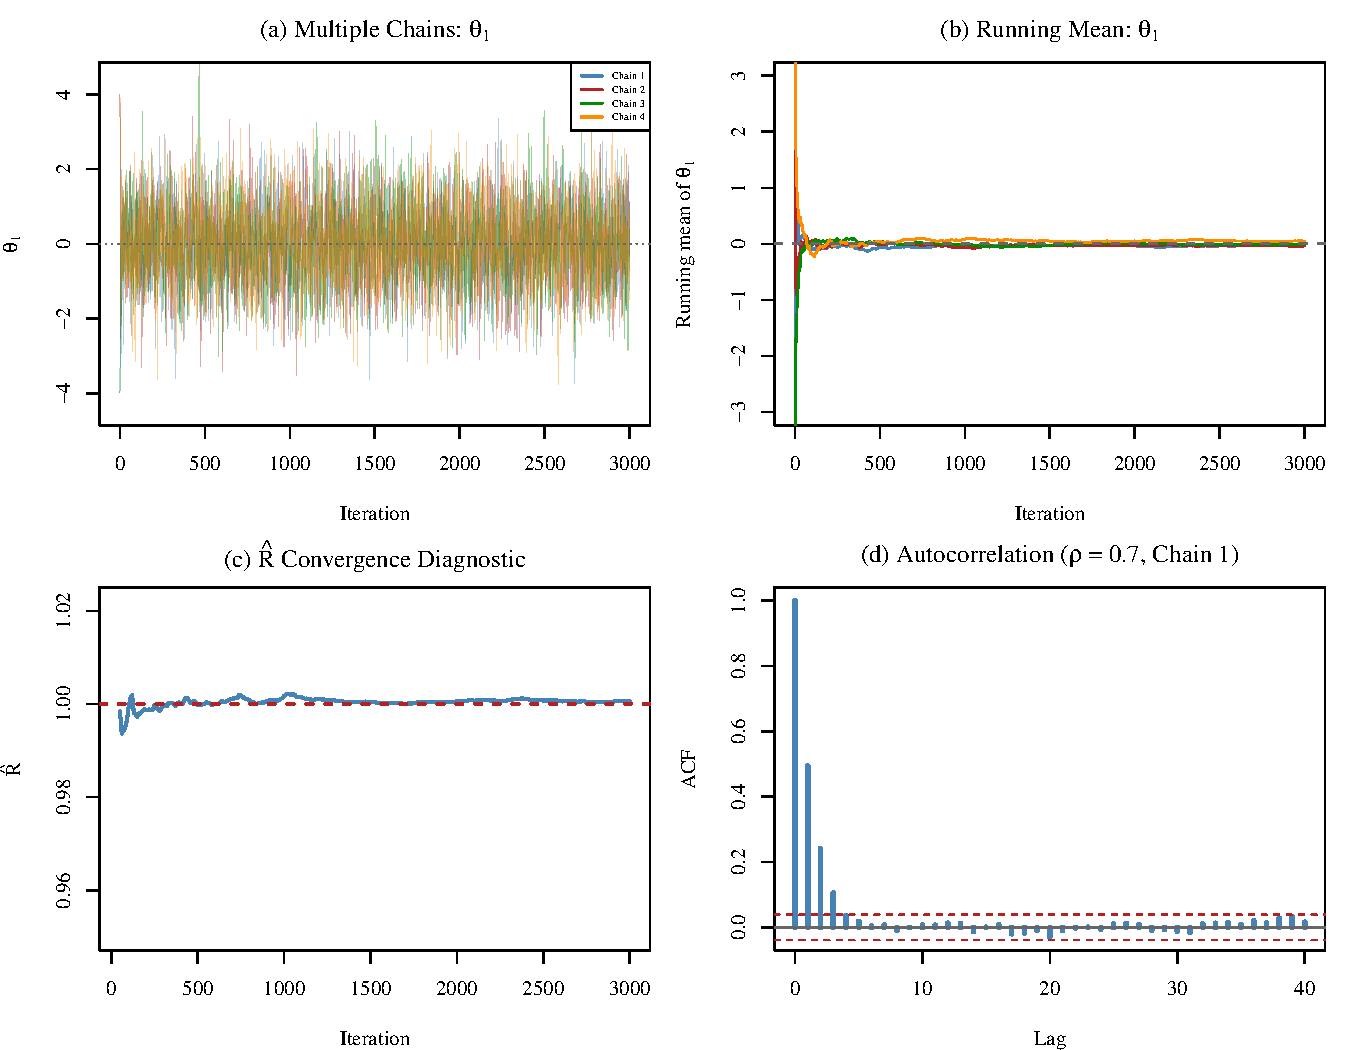
\includegraphics[width=\textwidth]{plots/fig_gibbs_diagnostics.pdf}
  \caption{%
    \textbf{(a)}~Four chains from dispersed starts, all converging.
    \textbf{(b)}~Running means stabilize near the true mean (0).
    \textbf{(c)}~$\hat{R}$ approaches 1.0 rapidly (orange dashed: 1.1 threshold).
    \textbf{(d)}~Autocorrelation function for Chain~1 (post-burn-in).
  }
  \label{fig:diagnostics}
\end{figure}

% ----------------------------------------------------------------
\section{Where Gibbs Sampling Fails}

\subsection{Multimodality}

Gibbs sampling moves through coordinate-wise updates.  If the target distribution has \textbf{well-separated modes}, the sampler can become trapped in one mode indefinitely.  This occurs because moving from one mode to another requires simultaneously changing multiple coordinates---something that axis-aligned updates cannot accomplish.

Figure~\ref{fig:failure}(a) shows a bimodal target with modes at $(3,3)$ and $(-3,-3)$ separated by a low-density ``valley.''  The modes are close enough that the sampler can occasionally jump between them.  Figure~\ref{fig:failure}(b) shows a more extreme case: modes at $(5,5)$ and $(-5,-5)$ with $\sigma = 0.5$.  Looking at the conditional $p(\theta_1 \mid \theta_2)$, when $\theta_2 = 5$, the conditional density at $\theta_1 = -5$ is essentially zero---the sampler \emph{never} proposes a jump to the other mode.

\subsection{Strong Posterior Correlations}

As demonstrated in Section~4, when the posterior has strong correlations (e.g., $\rho > 0.9$), the axis-aligned Gibbs updates can only make tiny incremental moves along the major axis of the distribution.  The effective sample size can drop to a few percent of the total iterations.

This is a general phenomenon: whenever the posterior has strong dependencies between
parameters---common in regression models with correlated predictors, or hierarchical
models with weak identification---Gibbs sampling mixes slowly.

\subsection{Intractable Full Conditionals}

Gibbs sampling \emph{requires} that all full conditional distributions be available in closed form (or at least easy to sample from).  When a conditional is not a standard distribution, one option is \textbf{Metropolis-within-Gibbs}: replace the exact Gibbs draw with a Metropolis--Hastings step for that component.  Alternatively, methods like Hamiltonian Monte Carlo (HMC) can update all parameters simultaneously, avoiding the coordinate-wise limitation entirely.

\paragraph{Figure~\ref{fig:failure}: Failure modes.}
Panel~(c) shows the $\theta_1$ trace for the well-separated bimodal case: the sampler remains stuck near~5 for the entire run, never visiting the mode at $-5$.  Panel~(d) quantifies the ESS degradation as a function of correlation $\rho$ in the bivariate normal.  At $\rho = 0.95$, ESS drops below $3\%$---meaning 10,000 Gibbs iterations yield fewer than 300 effectively independent samples.

\begin{figure}[H]
  \centering
  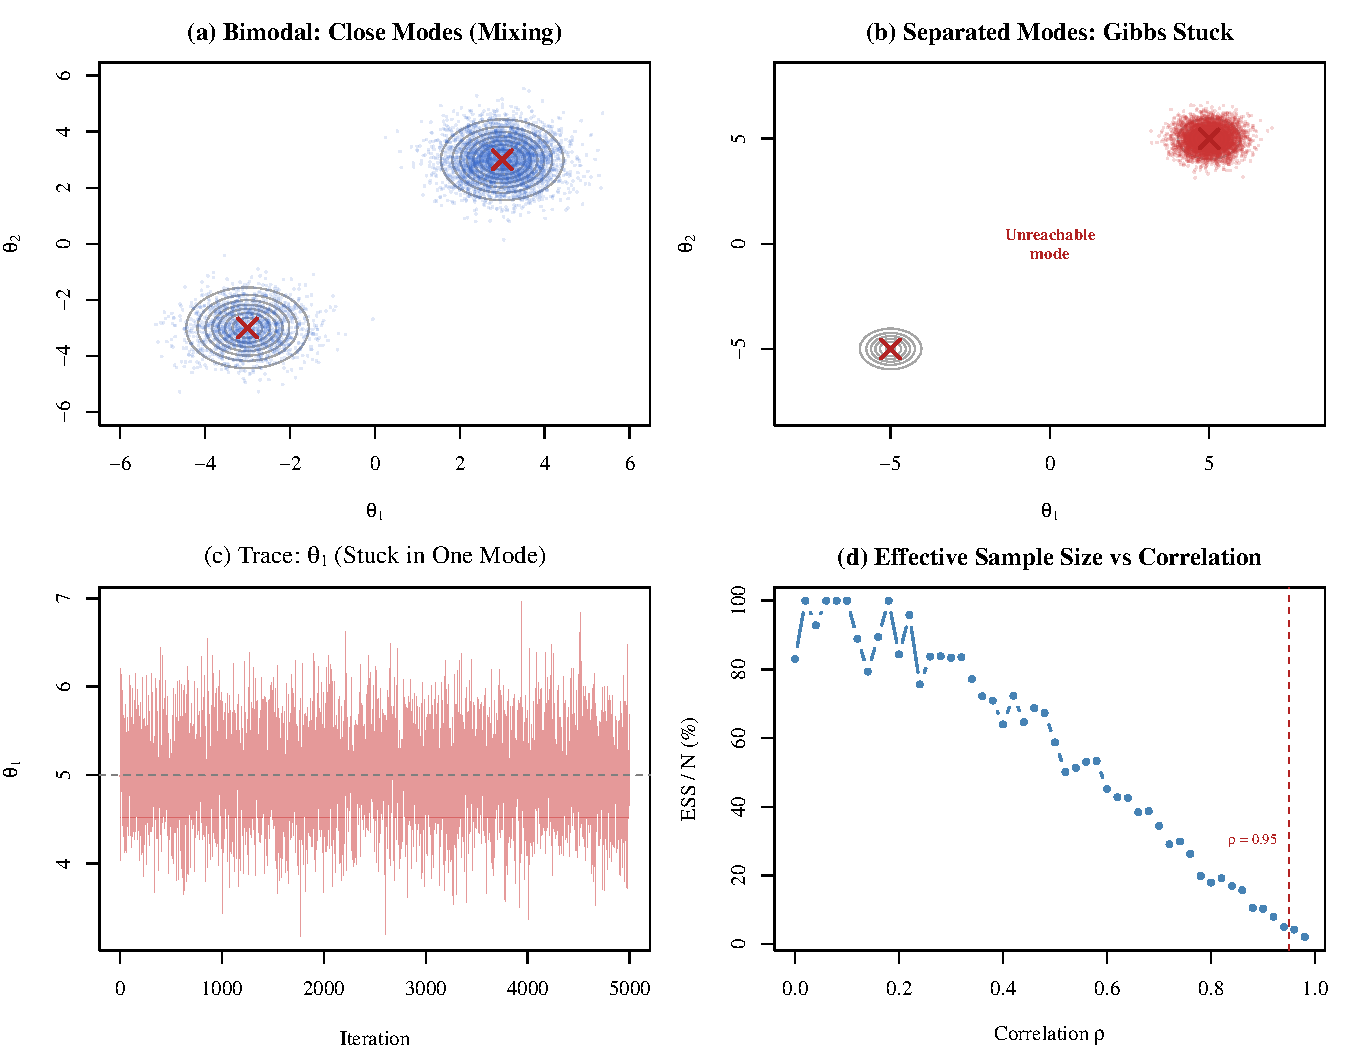
\includegraphics[width=\textwidth]{plots/fig_gibbs_failure.pdf}
  \caption{%
    \textbf{(a)}~Bimodal target with modes at $(\pm 3, \pm 3)$: Gibbs can mix (slowly) between modes.
    \textbf{(b)}~Modes at $(\pm 5, \pm 5)$: Gibbs is completely stuck in one mode.
    \textbf{(c)}~Trace plot showing the sampler trapped near $\theta_1 = 5$.
    \textbf{(d)}~ESS (as \% of $N$) plummets with increasing $\rho$.
  }
  \label{fig:failure}
\end{figure}

% ----------------------------------------------------------------
\section{Comparison with Other Methods}

\begin{table}[H]
\centering\small
\begin{tabular}{lcccc}
\toprule
& \textbf{Rejection} & \textbf{Importance} & \textbf{Metropolis--Hastings} & \textbf{Gibbs} \\
\midrule
Output & i.i.d.\ exact & Weighted & Correlated & Correlated \\
Acceptance rate & $1/c$ & N/A (all used) & Tunable & 100\% \\
Requires $c \cdot g \ge f$ & Yes & No & No & No \\
Norm.\ const.\ needed & Yes & No & No & No \\
Updates & Full vector & Full vector & Full / block & Component-wise \\
High-$d$ scaling & Fails & Degrades & Proposal-dependent & Correlation-dependent \\
Primary failure & Volume waste & Weight collapse & Poor tuning & Multimodality \\
\bottomrule
\end{tabular}
\caption{Comparison of Monte Carlo sampling methods.}
\label{tab:compare}
\end{table}

% ----------------------------------------------------------------
\section{Key Takeaways}

\begin{itemize}
  \item Gibbs sampling exploits the \textbf{conditional structure} of the target: instead of sampling from $p(\boldsymbol{\theta} \mid y)$ directly, it cycles through each component $\theta_j$ and draws from $p(\theta_j \mid \boldsymbol{\theta}_{-j}, y)$.
  \item The resulting Markov chain has $p(\boldsymbol{\theta} \mid y)$ as its \textbf{stationary distribution}, guaranteed by the invariance of conditional updates.
  \item Gibbs is a \textbf{special case of Metropolis--Hastings} with acceptance probability~1---every draw is accepted.
  \item The method is especially powerful for \textbf{conjugate hierarchical models} (e.g., the normal--normal model in BDA3, Chapters~3 and~5), where all full conditionals are standard distributions.
  \item \textbf{Strong posterior correlations} cause slow mixing: the axis-aligned updates can only make small steps along the correlated directions.  The effective sample size degrades as $n_{\text{eff}} \propto (1-\rho^2)$.
  \item \textbf{Multimodal targets} can trap the sampler in a single mode, since jumping between well-separated modes requires coordinated moves across multiple components.
  \item \textbf{Convergence diagnostics} ($\hat{R}$, trace plots, ESS) are essential.  Run multiple chains from dispersed starts and verify $\hat{R} < 1.1$ before trusting the results (BDA3, Section~11.4).
  \item When Gibbs sampling is inadequate (intractable conditionals, strong correlations, multimodality), consider \textbf{Metropolis-within-Gibbs}, Hamiltonian Monte Carlo, or other advanced MCMC methods.
\end{itemize}

\end{document}
